\documentclass{article}

\usepackage[english]{babel} % Multilanguage support for headings and such
\usepackage[backend=biber]{biblatex} % Bibliography support using biber
\usepackage[margin=32mm]{geometry} % Allows for customisation of margins and sizes
\usepackage[hidelinks]{hyperref} % Creates clickable links (+ hide the red box)
\usepackage{csquotes} % Improves the looks of quotes `' and ``'' (used by biblatex references)
\usepackage{tikz} % Allows fancy diagrams
\usepackage{graphicx} % Adds many graphic support tweaks

% Adds and improves mathematical notation
\usepackage{physics}
\usepackage{amsmath}
\usepackage{amssymb}


\addbibresource{main.bib}

\newcommand{\Exp}[1]{\big\langle #1 \big\rangle}
% some TikZ style shortcut definitions
\tikzstyle{order4}=[
    circle,
    inner sep = 2pt,
    draw = green,
    fill = green,
]
\tikzstyle{maybe_order4} = [
    circle,
    inner sep = 2pt,
    draw = green,
    fill = white,
]
\tikzstyle{triangle}=[
    draw = #1,
    fill = #1!50,
    ultra thick,
]
\tikzstyle{edge} = [
    draw = #1,
    ultra thick
]
\interfootnotelinepenalty=10000

\title{{\huge 2D Causal Dynamical Triangulations} \\ {\Large using Markov-chain Monte Carlo methods}}
\author{\textit{Institute for Mathematics, Astrophysics and Particle Physics, Radboud University} \\[1mm] T.B.H. Gerstel \hspace{1cm} J.G.R. van der Duin}

\begin{document}

\maketitle

\begin{abstract} % (including research question and main results)
    Causal Dynamical Triangulation is a method to regularise the gravitational path integral by building a piece-wise flat spacetime from simplices.
    The goal of this project is to create an efficient 2D numerical model which can generate these piece-wise flat spacetimes or triangulations, and to use these to measure observables in 2D CDT using Monte Carlo methods to verify the validity of the model by comparison with theory.
    The simulational model is created in Rust and uses a Markov-chain to generate random triangulations. Data analysis is done in Python.
    Using this model, we are able to measure the length covariance on a two-dimensional torus for different triangulation sizes of up to 100,000 triangles and demonstrate that the theoretical expectation is within the statistical error our results.
\end{abstract}

\newpage

\section{Introduction}
% Introduction to the research area and research question
\subsection{Quantum Gravity}

A field of theoretical physics which still has many open questions is quantum gravity. One may notice that "quantum gravity" consists of two words: "quantum" and "gravity". The "gravity" aspect is quite well understood, and its content can be compactly summarised in the Einstein-Hilbert action
\begin{equation}
    S[g_{\mu \nu}]
    =
    \frac{1}{16 \pi G}
    \int_{\mathcal{M}} \dd[d]{x} \sqrt{-g(x)}
    \qty(R(x) - 2 \Lambda)
    ,
\end{equation}
where the integration is over the entire $d$-dimensional spacetime manifold $\mathcal{M}$. Here $R(x)$ is the Ricci curvature scalar, $g(x)$ is the determinant of the metric tensor $g_{\mu \nu}$, $G$ is Newton's gravitational constant and $\Lambda$ is the cosmological constant. Classical equations of motion can then be obtained via a variational principle by solving $\variation{S} = 0$.

A common approach to add the "quantum" aspect to any classical theory is by introducing a path integral. Since in our case the classical action is a functional of the metric $g_{\mu \nu}$, the path integral is given by
\begin{equation}
    Z
    =
    \int \frac{\mathcal{D}[g_{\mu \nu}]}{\text{Diff}(\mathcal{M})}
    e^{i S[g_{\mu \nu}]}
    .
\end{equation}
But what does this actually mean? How could one explicitly carry out this integration?

\subsection{Causal Dynamical Triangulations}

We somewhat avoid these questions by adopting a certain regularisation approach, namely Causal Dynamical Triangulations (CDT). Instead of trying to integrate over all continuously curved manifolds, we sum over piecewise flat manifolds that are constructed by gluing a certain class of flat building blocks together. In particular, these building blocks will be $d$-dimensional regular simplices with a flat Minkowskian interior. These simplices have squared edge lengths fixed at $\pm a^2$ (allowing space- and timelike edges), where $a$ is also a regularisation parameter. We foliate the manifold into $T$ $(d - 1)$-dimensional timeslices, labelled by $t = 0, \ldots T - 1$, connected by a single layer of $d$-dimensional simplices. Different manifolds can be obtained by changing the way simplices are connected. Now the regularised path integral can be written as
\begin{equation}
    Z
    =
    \sum_{T \in \mathcal{T}} \frac{1}{C(T)} e^{i S[T]}
    ,
\end{equation}
where the summation is over all triangulations. Here $S[T]$ is the action and $C(T)$ is a symmetry factor for a given triangulation $T$\footnote{Unfortunately the symbol $T$ is the most natural choice for denoting both a particular triangulation, as well as the number of timeslices contained in such a triangulation. Hopefully it will be clear from context which of the two is used.}.

\paragraph{Simplifications} To simplify matters, we only consider 2-dimensional spacetimes with periodic boundaries. The resulting topology is that of a 2-torus. Note that in this case each timeslice is just a ring of spacelike edges. The number of spacelike edges in timeslice $t$ is denoted by $\ell(t)$. With this in mind, we make a few useful observations:
\begin{itemize}
    \item All triangles have equal volume, so the total volume is proportional to the number of triangles.
    \item The manifold is piecewise flat, meaning a Wick rotation is well-defined.
    \item In 2 dimensions the integrated scalar curvature is constant and therefore irrelevant for the dynamics.
\end{itemize}
Using these observations we find that the Euclidean action for a 2-dimensional triangulation $T$ is \cite{2012}
\begin{equation}
    S[T] = \lambda N(T),
\end{equation}
where $\lambda$ is a dimensionless constant related to the cosmological constant $\Lambda$. For now we can just interpret it as a model parameter.

To simplify the symmetry factor $C(T)$ we label all triangles\footnote{This is of course also convenient when encoding the triangulation in a computer.}. Each triangulation can be labelled in $N(T)!$ ways, so the Euclidean path integral (or partition sum) becomes
\begin{equation}
    Z
    =
    \sum_{T_\ell \in \mathcal{T}_\ell} \frac{1}{N(T_\ell)!} e^{- \lambda N(T_\ell)}
    ,
\end{equation}
where the summation is now over all labelled triangulations. It is possible to split the partition sum into contributions with a certain number of triangles, as follows
\begin{equation}\label{eq:part_sum}
    Z
    =
    \sum_{N = 0}^\infty \Omega(N) \frac{e^{- \lambda N}}{N!}
    ,
\end{equation}
where $\Omega(N)$ denotes the number of labelled triangulations with $N$ triangles.

\subsection{Continuum Limit}

Since we are studying a regularised path integral, it is interesting to consider what happens if we let the regularisation parameter $a$ go to zero. In this continuum limit lengths and timespans scale as $L = a \ell$ and $T = a t$,respectively\footnote{Indeed, unfortunately there is yet another quantity for which $T$ is the most natural (and conventional) choice.}. The parameter $\lambda$ undergoes an additive renormalisation
\begin{equation}
    \Lambda = \frac{\lambda - \ln 2}{a^2}
    .
\end{equation}

In order to extract information from this continuum limit, it would be useful to have an expression for the continuum propagator. In this context, the propagator is proportional to the probability that a spacelike slice of length $L_1$ evolves into a slice of length $L_2$ over some time interval of size $T$. Fortunately, an analytic expression for this propagator has been found, and it is given by the beautiful expression \cite{1998}
\begin{equation}
    G_\Lambda(L_1, L_2, T)
    =
    \frac{
        e^{-\qty[\coth \sqrt{\Lambda} T] \sqrt{\Lambda} (L_1 + L_2)}
    }{
        \sinh \sqrt{\Lambda} T
    }
    \frac{\sqrt{\Lambda L_1 L_2}}{L_2}
    I_1 \qty(\frac{2 \sqrt{\Lambda L_1 L_2}}{\sinh \sqrt{\Lambda} T})
    ,
\end{equation}
where $I_1(x)$ is a modified Bessel function of the first kind.

To be able to extract information from this propagator, we look at the limit $\sqrt{\Lambda} T \gg 1$. In this regime, we can approximate the propagator as
\begin{equation}
    G_\Lambda(L_1, L_2, T)
    \approx
    4 \Lambda L_1 e^{-\sqrt{\Lambda} (L_1 + L_2 + T)}
    .
\end{equation}
In the limits $\sqrt{\Lambda} T_1, \sqrt{\Lambda} T_2 \gg 1$, the probability distribution\footnote{Note that due to the large time regime we restrict ourselves to, we expect this distribution to be independent of the time at which $L$ is considered.} for the length $L$ is given by
\begin{equation}
    p(L)
    =
    \frac{
        G_\Lambda(L_1, L, T_1)
        G_\Lambda(L, L_2, T_2)
    }{
        \int_0^\infty \dd{L}
        G_\Lambda(L_1, L, T_1)
        G_\Lambda(L, L_2, T_2)
    }
    =
    4 \Lambda L e^{-2 \sqrt{\Lambda} L}
    .
\end{equation}
We can then of course compute the mean of this probability distribution. It is given by
\begin{equation}\label{eq:exp_ell}
    \ev{L} = \frac{1}{\sqrt{\Lambda}}.
\end{equation}
And its variance is given by
\begin{equation}\label{eq:std_ell}
    \sigma_L^2 = \ev{L^2} - \ev{L}^2 = \frac{1}{2 \Lambda}
    .
\end{equation}

The quantities we have discussed so far only describe the global behaviour of the typical length $L$ of a spacelike slice in our universe. While these provide useful checks on our model, we would also like to consider more interesting quantities that show how different lengths are related in time. In particular, we would like to compute the autocovariance of $L$ as a function of $T$. To this end we compute (in the limits $\sqrt{\Lambda} T_1, \sqrt{\Lambda} T_2 \gg 1$ but with $\sqrt{\Lambda} T = \mathcal{O}(1)$) the joint probability distribution
\begin{equation}
    p(L(0), L(T); T)
    =
    \frac{
        G_\Lambda(L_1, L(0), T_1)
        G_\Lambda(L(0), L(T), T)
        G_\Lambda(L(T), L_2, T_2)
    }{
        \int_0^\infty \dd{L(0)} \int_0^\infty \dd{L(T)}
        G_\Lambda(L_1, L(0), T_1)
        G_\Lambda(L(0), L(T), T)
        G_\Lambda(L(T), L_2, T_2)
    }
    ,
\end{equation}
where $T > 0$. From this probability distribution we can compute the expectation value
\begin{equation}
    \ev{L(0) L(T)}(T)
    =
    \frac{e^{-2 \sqrt{\Lambda} \abs{T}}}{2 \Lambda} + \frac{1}{\Lambda}
    ,
\end{equation}
where the absolute value comes from the fact that by symmetry $T$ and $-T$ should give the same result. Then we find that the autocovariance is
\begin{equation}\label{eq:cov_ell}
    \gamma_L(T)
    =
    \ev{L(0) L(T)} - \ev{L(0)} \ev{L(T)}
    =
    \frac{e^{-2 \sqrt{\Lambda} \abs{T}}}{2 \Lambda}
    .
\end{equation}

Later on these quantities will be measured on the discrete model. In order to compare to these quantities, one needs to make the substitutions $L = a \ell$ and $T = a t$. The observables are rescaled in the obvious way as $\sigma_L = a \sigma_\ell$ and $\gamma_L = a^2 \gamma_\ell$, such that all factors of $a$ match. The cosmological constant $\Lambda$ can be related using Eq. \eqref{eq:exp_ell}, resulting in
\begin{equation}
    \Lambda = \frac{1}{a^2 \ev{\ell}^2}
    .
\end{equation}
However, in our implementation of the discrete model $\ev{\ell}$ will be fixed and its value must be provided as an input parameter $L$\footnote{Yet another unfortunate naming convention: in this context $L$ is a discrete parameter provided as an input for the model, whereas before it denoted the continuous length of some spacelike slice.} (See section \ref{sec:implementation}).


\section{Methods}
% explaining the algorithms and why they work
One could imagine trying to sample triangulations according to \eqref{eq:part_sum}.
However, this is not very practical. It turns out that $\Omega(n) \sim n! 2^n$. This means that for $\lambda > \ln 2$ large volumes are suppresed so that a typical triangulation will contain only a handful of triangles.
However, when $\lambda < \ln 2$ the partition sum \eqref{eq:part_sum} diverges and the problem is ill-defined.

A solution is to consider only triangulations of a certain fixed volume at a time.
An advantage of this approach is that the desired distribution becomes uniform, since the weight of each triangulation depends only on its volume.
In practice, this can be obtained by using update rules that keep the number of triangles fixed.

\subsection{Update rules}
% Should we also include alternative update rules we attempted? And why the don't work? It does show the amount of work and consideration we put into constcuting an effective MCMC simulation, but Im not sure.

\subsection{Observables} \label{sec:observables}
% Explain choice of observables, possibly alternatives that were considered but not measured
% Maybe also explain how lengthprofile is obtained from implementation, as this is not entirely trivial and Timothy asked about this after the presentation
Finding good observables to measure is quite challenging in (C)DT. This may partly be due to a lack of experimental data to compare simulations to.
But also where many Monte Carlo simulations in physics are concerned with describing the behaviour of fields on a lattice, naturally giving some combination of the field values as observables,
there is no such field in CDT but the lattice itself should provide the information of interest.

The chosen observables can of course not depend on any details of the implementation, like the use of labelling in our implementation.
And for an observable to be of physical interest it should also have a well-defined limit for the amount of triangles $N \rightarrow \infty$.
Observables that are often looked at are different notions of dimension, notably the \emph{spectral dimension} \cite{2012} and \emph{Hausdorff dimension} \cite{1998, 2012}, the latter of which has also been discussed in the case of Dynamical Triangulation in the course Monte Carlo Techniques. And a newer observable of interest is a certain notion of \emph{Quantum Curvature} -- a sort of extended notion of Ricci curvature which can be applied to the used triangulations and obeys a proper limit \cite{brunekreef2021}.

However since the focus of this project was more in the implementation of a Markov Chain Monte Carlo simulation, and the measurements and analysis of these observables is somewhat involved, we only consider observables that are derived from the volume of the space-like slices.
This means that in $1 + 1$D CDT we look at the \emph{length}, that is the amount of edges or equivalently the amount of vertices in a time-slice, at different times; this we call the \emph{length profile} $\ell(t)$

\paragraph{Length profile}
The length profile itself still depends on a certain choice of origin in $t$, while we consider a toroidal topology so any there is no preferred origin. Thus, any observable should have some sort of averaging over $t$.

The simplest observable to consider is the average of $\ell(t)$, but this is trivially $L$ since the total amount timeslices and triangles and thus vertices is kept fixed.
So the simplest non-trivial observable we can think of is the standard deviation $\sigma_\ell$ of the length profile $\ell(t)$:
\begin{equation}
    \sigma_\ell^2 = \frac{1}{T} \sum_{t = 1}^{T} \Big(\ell(t) - L\Big)^2,
\end{equation}
using the usual definition of the population variance.

%TODO possibly we want to use a different notion of length correlation
But $\sigma_\ell$ does not contain any information of the relation of lengths between different times $t$.
So an arguably more interesting observable is what we call the \emph{length correlation}:
\begin{equation}
    \rho_\ell(t) = \frac{1}{T \sigma_\ell^2} \sum_{t_0 = 1}^{T} \qty(\ell(t_0) - L)\qty(\ell(t_0 + t) - L),
\end{equation}
where this correlation is normalised such that $\rho_\ell(0) = 1$.
Note that the length correlation is still a function of $t$ but this $t$ is the time difference between two time-slices, so there is no origin dependence.

Both observables $\sigma_\ell$ and $\rho_\ell(t)$ do diverge for $N \rightarrow \infty$ as they will scale with $N$.
How they will scale is at this point not known, but we hope they will scale in a well-behaved way such that with proper rescaling these observables may have a well-defined limit.

\subsection{Implementation}
% This was probably the most substantional amount of work of this project, so I think this should be reflected in the size of this part
% Also here I'm not sure whether to include the failed attempts?

\paragraph{Length profile}
% Explain how length profile was obtained from implementation

\section{Results and Discussion}
% Including plots and final quantitative outcomes with errors
% Brief overview of the observables that are measured
The observables we measured in the $1 + 1$D CDT model are the \emph{standard deviation} of the length profile $\sigma_\ell$ and the \emph{length covariance} $\rho_\ell(t)$ as introduced in section \ref{sec:observables}.
In this section we will present and discuss the results found for these observables.

\subsection{Pre-analysis}
% Determination of the equilibration time and correlation time
Before the actual measurements can be performed some data analysis need to be done beforehand.

\paragraph{Equilibration}
To be able to take measurements of the wanted observables in the Markov-chain Monte Carlo simulation the system needs to be thermalised. Which is to say that the system should be in a `typical' state, such that the expectation value of an observable at any timestep in the simulation is the same as that of any other.
We start the system in a non-typical, flat spacetime, so it takes some Markov-chain steps before the system is in equilibrium.
We want to only start measurements after this \emph{equilibration time}, so we need to estimate it to know when to start measuring.

Preferably, one uses the observable of interest to determine the equilibration time, however it is very difficult to quantify when a function like $\rho_\ell(t)$ has thermalised. So for both observables we determine the equilibration time using $\sigma_\ell$.
To determine when the system has equilibrated in terms of $\sigma_\ell$ we fit a function which converges exponentially towards the average value:
$\sigma(t) = \hat\sigma \qty(1 - e^{t/t_\text{eq}})$, where $t$ here is the Monte Carlo simulation time, and $t_\text{eq}$ then defined equilibration time.
This works well because initially $\sigma_\ell = 0$ as the starting triangulation is flat, which over time changed to fluctuating around some mean value.
\begin{figure}[ht]
    \centering
    \begin{minipage}[t]{0.47\linewidth}
        \centering
        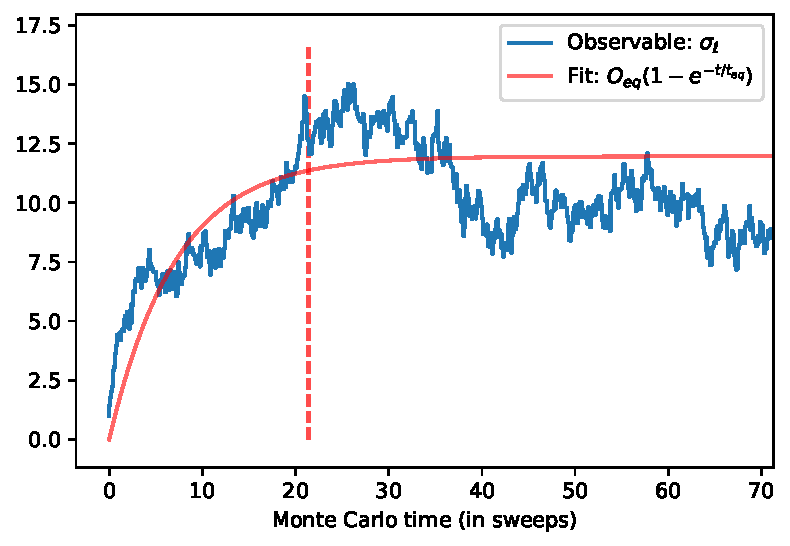
\includegraphics[width=0.95\linewidth]{img/teq_thermalisation.pdf}
        \caption{Visualisation of determination of thermalisation by fitting an exponential convergence. \textit{Marking at $3t_\text{eq}$}}
        \label{fig:thermalisation}
    \end{minipage}
    \hfill
    \begin{minipage}[t]{0.48\linewidth}
        \centering
        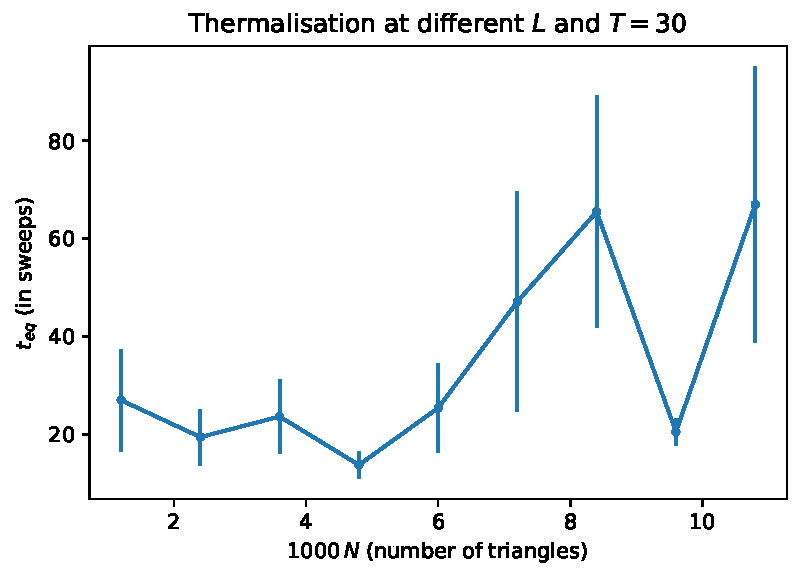
\includegraphics[width=0.95\linewidth]{img/teq-Ldep.pdf}
        \caption{Equilibration time for different sizes of $L$, based on 10 samples for each system size. Determined at move ratio $r=0.4$.}
        \label{fig:teq_Ldep}
    \end{minipage}
\end{figure}
This fitting procedure is visualised in Fig. \ref{fig:thermalisation}.
So using this method we can estimate the equilibration time given a trace of $\sigma_\ell$.

Then instead of determining the equilibration time for every system we wish to measure, we attempted to determine the dependence of the equilibration time on different system sizes.
To do this we measured $t_\text{eq}$ for different values of $L$ and repeated each measurement 10 times to obtain more accurate results and get an estimate of the error in the results.
This yields the results in terms of sweeps presented in Fig. \ref{fig:teq_Ldep} (note that $N = 2 L T$).

The found results show no clear dependence of $t_\text{eq}$ on the system size, and since we only wish to obtain an order estimate of it seems reasonable to assume that \emph{in terms of sweeps} the equilibration time is independent of the system size.
We then take the equilibration time to be $t_\text{eq} = 200 \, \text{sweeps}$ for all simulations to be safe.
This is a very crude approximation of the equilibration time, but since $200 \, \text{sweeps}$ is relatively small it seems unnecessary to put more work in a better estimate of the equilibration time.


\paragraph{Autocorrelation}
Once the system has thermalised, we can start to take measurements of the observables of interest.
However, after a single simulation timestep the newly obtained state is still very similar to the previous state, thus observables measured in these different states are by no means independent; they are in fact highly correlated.
Having many correlated measurements is not useful as they do not make the final estimate better, and take up a lot of unnecessary space and computation time.
Moreover, to be able to make and estimate of the error in the final results, it is crucial to know the correlation between measurements.

To estimate the correlation time we will again use $\sigma_\ell$ as observable, as this is much easier than using the function $\rho_\ell(t)$.
The correlation time is then estimated as usual by determining the \emph{autocorrelation} of the standard deviation observable over for time:
\begin{equation*}
    \rho(t) = \frac{1}{Z} \, \sum_{i = 1}^{M - t} \qty(\sigma_{\ell, i} - \bar{\sigma}_\ell) \qty(\sigma_{\ell, i + t} - \bar{\sigma}_\ell),
\end{equation*}
where $\sigma_{\ell, i}$ is the $i$th measurement in a set of $M$ measurements of $\sigma_\ell$, $\bar \sigma_\ell$ is the sample average, and $Z$ is a normalisation factor such that $\rho(0) = 1$.

Now for long enough measurements we expect that the autocorrelation follows exponential decay with which we can define the correlation time $t_\text{cor}$, such that $\rho(t) \approx \exp(- t / t_\text{cor})$.
So to estimate $t_\text{cor}$ we simulate a long trace of $\sigma_\ell$ and fit an exponential decay to the autocorrelation of that trace.
To estimate the error on the estimate of the correlation time we can repeat the measurements several times; or we can simulate a very long trace and divide the trace up in batches which we treat as separate measurements, which simply saves on thermalisation.

We would like the autocorrelation to be as small as possible. So we can tune the introduced move ratio $r$ such that the autocorrelation is minimized.
To achieve this we estimate the autocorrelation for different move ratio's, the results of which are displayed in Fig. \ref{fig:tcor_rdep}.
\begin{figure}[ht]
    \centering
    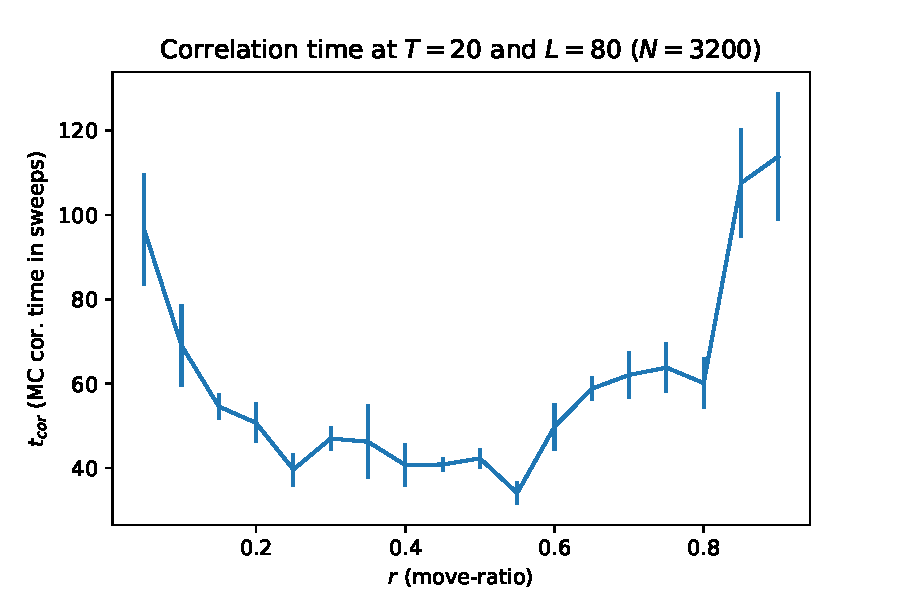
\includegraphics[width=0.7\linewidth]{img/tcor_r_t20_l80.pdf}
    \caption{Correlation time as function of the move-ratio.}
    \label{fig:tcor_rdep}
\end{figure}
From this figure one can clearly see that move rates close to $0.0$ or $1.0$ have a very long correlation time.
This makes sense as only flip moves cannot change the length profile at all and without flip moves there are no new places created for shard moves to occur, so the shards move around between the same places.
It also appears that the correlation time is not very sensitive to the move rate $r$, as the correlation time estimate remains roughly constant for $r$ between $0.3$ and $0.5$.
So it seems save to simply pick $r = 0.4$ as there is no need to tune the rate to a very specific value.

Then finally we wish to estimate the dependence of the correlation time on the system size. To do this we estimate the correlation time for multiple system sizes like was done for the equilibration time.
We measured the correlation for different values of $T$ and $L$ keeping the other constant. The results of these measurements are presented in Fig. \ref{fig:tcor_L} and \ref{fig:tcor_T}.
\begin{figure}
    \centering
    \begin{minipage}{0.48\linewidth}
        \centering
        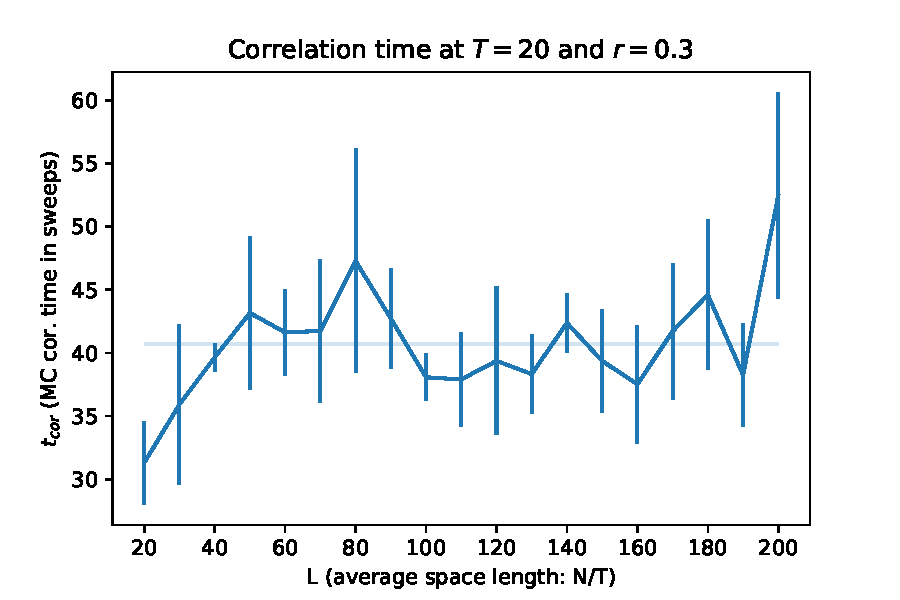
\includegraphics[width=1.0\linewidth]{img/tcor_l_t20_r0.3.pdf}
        \caption{Correlation time at $T = 20$ for different $L$, with corresponding fit.}
        \label{fig:tcor_L}
    \end{minipage}
    \hfill
    \begin{minipage}{0.48\linewidth}
        \centering
        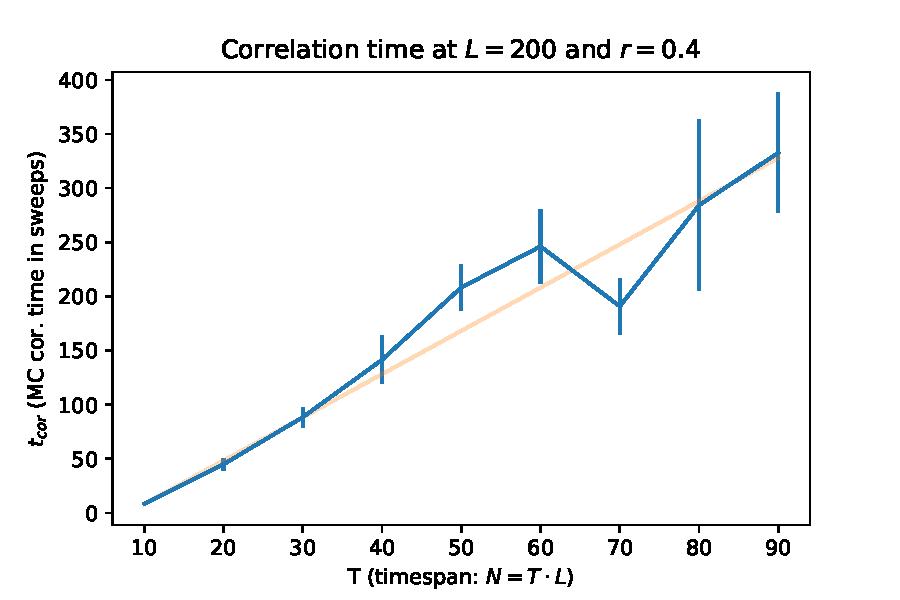
\includegraphics[width=1.0\linewidth]{img/tcor_t_l200_r0.4.pdf}
        \caption{Correlation time at $L = 200$ for different $T$, with corresponding fit.}
        \label{fig:tcor_T}
    \end{minipage}
\end{figure}
From Fig. \ref{fig:tcor_L} it seems that \emph{in terms of sweeps} the correlation time is roughly constant under $L$ and can at $T = 20$ taken to be $t_\text{cor} = 41 \, \text{sweeps}$.
However, under changing $T$ the $t_\text{cor}$ seems to be growing roughly linearly, giving the crude approximation $t_\text{cor} \approx 4\, (T - 10)$ that can be use as an estimate for the correlation time for a wanted system size.
This estimate is very crude, but keep in mind that the final results do not actually depend on this measurement of the correlation time. It helps to know the correlation time to be able to only save relevant data, but it will not affect the final results.
So this approximation is sufficient for the purposes of this simulation.

Note that this linear scaling in $T$ of the correlation time (in terms of sweeps), means that the amount of Markov-chain Monte Carlo steps grows like $N^{3/2}$ for a constant ratio $T/L$. This scaling means that our computation time will increase like $N^{3/2}$ the system size is increased, and puts a limit on the system sizes that can be measured.


\subsection{Measurements}
With the system in equilibrium and an estimate for the correlation time, we can start to measure observables.
We wish to compare the measured standard deviation and covariance to the theoretical expectation of 2D CDT, as determined in the $T \rightarrow \infty$ limit.
To simulate measurements in this limit we wish to choose $T$ such that $L \ll T$; in this case we use $T = 20 \, L$ as larger values of $T$ have a large impact on computation time.
We can then compute the \emph{length profile} $\ell(t)$ over a range of $L$ values.
Within time constraints, we were able to measure a range of $L = 15, 20, \dots, 50$; we performed $100$ measurements on each $L$ at $\sqrt{0.4 \, N} \, \text{sweep}$ intervals, which is chosen as the correlation time appears to be roughly $t_\text{cor} \approx 3 \sqrt{N} \text{sweep}$\footnote{This is different from the estimate of $t_\text{cor}$ determined before, this discrepancy is further discussed in \ref{sec:discussion}} at this $T/L$ ratio.

\paragraph{Standard deviation}
% Presentation of the results of the standard deviation of the length profile
The data from the simulation can be analysed to obtain estimates of $\sigma_\ell$, and using Eq. \eqref{eq:std_ell} estimates for $\Lambda$.
From Eq. \eqref{eq:exp_ell} we expect the cosmological constant and equivalently the standard deviation to depend on the system size like:
\begin{equation}\label{eq:std_theory}
    \Exp{\Lambda} = \frac{1}{L^2}, \qquad \Exp{\sigma_\ell} = \frac{L}{\sqrt{2}} \approx 0.71 \, L.
\end{equation}

To estimate $\sigma_\ell$ and the error in the estimation the standard deviation is computed from the length profile, according to Eq. \eqref{eq:std_meas}, for every measurement after which \emph{batching}\footnote{In \emph{batching} correlated measurements are divided in $M$ batches larger than $t_\text{cor}$ and each batch is averaged to obtain $M$ uncorrelated measurements that are considered \emph{independent identically distributed}.
The observable is than estimated by taking the mean of the obtained measurements, and the error is estimated by the standard deviation of the obtained measurements divided by $\sqrt{M - 1}.$
} is used. For these measurements 10 batches were used, and the batches are checked to have no not significant autocorrelation.
The results of this analysis for the different values of $L$ is presented in Fig. \ref{fig:std_estimate} together with a power-law fit ($a \, e^{\nu}$).
\begin{figure}[ht]
    \begin{minipage}[t]{0.49\linewidth}
        \centering
        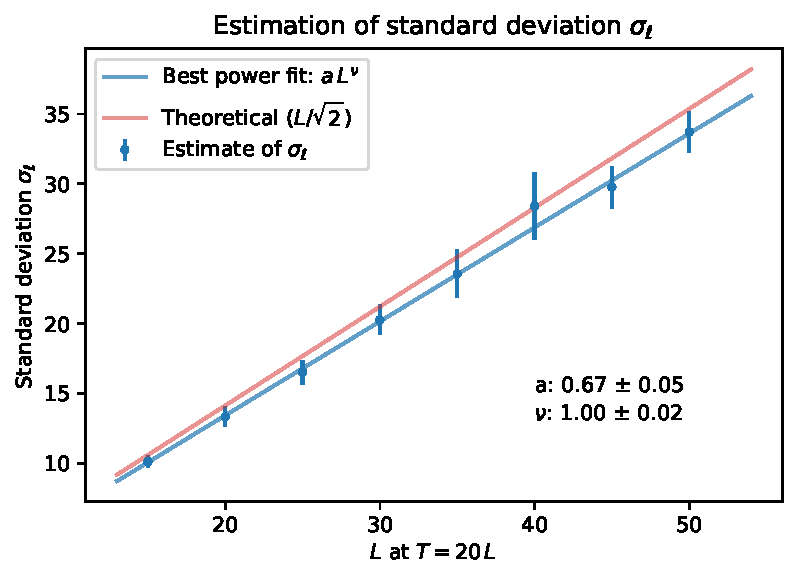
\includegraphics[width=\linewidth]{img/std_estimate.pdf}
        \caption{Measurement results of $\sigma_\ell$ for different system sizes $L$, with power-law fit and theoretical expectation.}
        \label{fig:std_estimate}
    \end{minipage}
    \hfill
    \begin{minipage}[t]{0.49\linewidth}
        \centering
        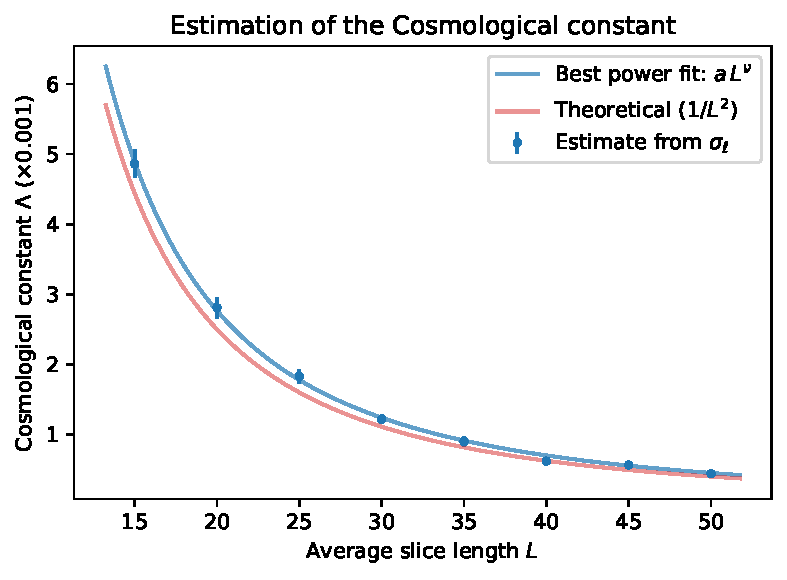
\includegraphics[width=\linewidth]{img/Lambda_estimate.pdf}
        \caption{Estimates for $\Lambda$ based on the $\sigma_\ell$ measurements, with power-law fit and theoretical expectation.}
        \label{fig:Lambda_estimate}
    \end{minipage}
\end{figure}

For the fit is found that $a = 0.67 \pm 0.05$ and $\nu = 1.00 \pm 0.02$, thus we see that as expected by Eq. \eqref{eq:std_theory} $\sigma_\ell$ indeed grows linearly in $L$ with good accuracy and $0.71$ falls within the $68\%$ confidence interval of $a$.
However, from the plot in Fig. \ref{eq:std_ell} it seems that the measurements systematically underestimate the standard deviation.
Since the theoretical result falls within the error, this may simply be coincidence and requires more measurements to decrease the error.
However, this is likely a systematic error made due to having finite $T$, as $\ell(t)$ can only change a finite amount between adjacent timeslices, so having a finite $T$ means that $\ell(t)$ can possibly not fluctuate as far from $L$ as it could for $T \rightarrow \infty$.
To investigate this, and in general the effect of different $T/L$ ratio's, these measurements should be repeated for different values of $T$.
It would be very interesting to get a better view on how the results convergence under increasing $L$, but unfortunately we could not measure this within the time constraint of this project.

From the estimates of $\sigma_\ell$ we can also estimate the cosmological constant $\Lambda$ of the simulated systems, which is used later. This is done simply by the transformation of stochastic variables $\Lambda = 1/2\sigma_\ell^2$, and transforming the mean value and error as usual.
The resulting $\Lambda$ estimates for different $L$ are displayed in Fig. \ref{fig:Lambda_estimate}. From this no real additional information can be extracted as it is simply a transformation, but we can confirm that the cosmological constant closely relates to $L$ with the expected relation \eqref{eq:std_theory}.



\paragraph{Length covariance}
% Presentation of the results of the analysis of the length correlation of the length profile
Next we can also analyse the \emph{length covariance} $\rho_\ell(t)$ from the measured length profiles, and compare then to the theoretical covariance \eqref{eq:cov_ell}, now using the discrete $t$ and $\Lambda$ instead.
We compute the covariance for every measurement according to Eq. \eqref{eq:cov_meas} and use the same \emph{batching} method to estimate the covariance and error at every $t$.
The resulting estimates are displayed in Fig. \ref{fig:cov_plot} with $68\%$ confidence intervals.
\begin{figure}[ht]
    \begin{minipage}[t]{0.49\linewidth}
        \centering
        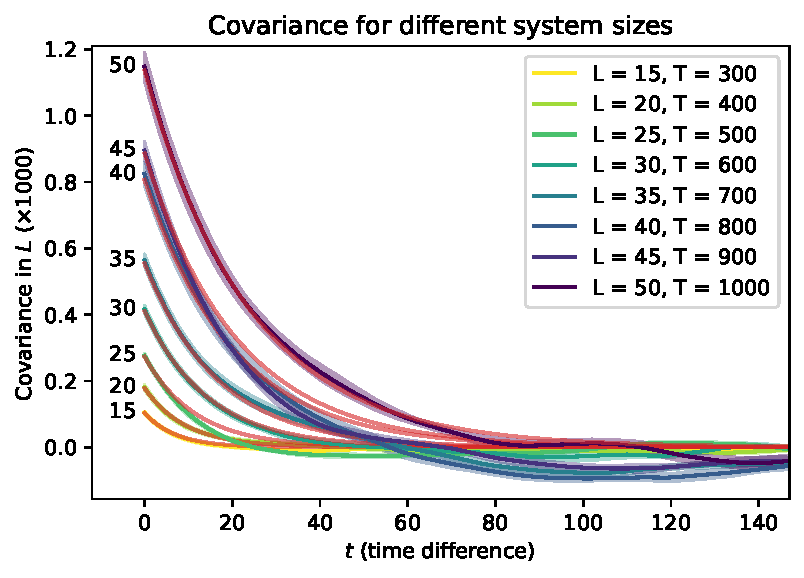
\includegraphics[width=\linewidth]{img/cov_L.pdf}
        \caption{Estimates of the length covariance, labelled by $L$ and show in units of $1000$.}
        \label{fig:cov_plot}
    \end{minipage}
    \hfill
    \begin{minipage}[t]{0.49\linewidth}
        \centering
        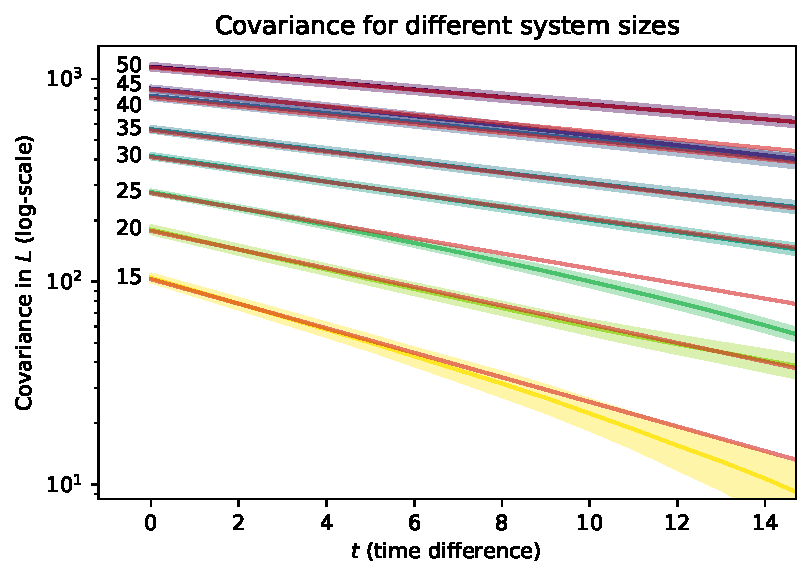
\includegraphics[width=\linewidth]{img/cov_L_log.pdf}
        \caption{Log plot of the length covariance, labelled by $L$ and including theoretical covariance.}
        \label{fig:cov_log_plot}
    \end{minipage}
\end{figure}

Now, to compare these measurement results to theory it is important to realise that Eq. \eqref{eq:cov_ell} are only valid for\footnote{Again note that here $T$ is the amount of timeslices and $t$ the discrete time difference corresponding to the continuous time difference $T$ in Eq. \eqref{eq:cov_ell}} $t \ll T$, which makes it difficult to fit a general exponential through the measured covariance as this exponential relation is only expected to hold for small $t$.
An alternative is to visualise the theoretical covariance alongside the measured covariance such that we can at least visually inspect whether the data matches the expected results.
To plot the theoretical covariance \eqref{eq:cov_ell}, a value for $\Lambda$ is required.
The obvious choice is to let $\Lambda = 1/L^2$ as is theoretically expected.
However, we know from the measurements of $\sigma_\ell$ that it is underestimated, and since $\sigma_\ell^2$ is precisely the normalisation of the covariance using $\Lambda = 1/L^2$ would mean we have this underestimation for all $t$.
And because we already analysed $\sigma_\ell$, the absolute magnitude of the covariance is not that interesting; it is much more interesting to look whether the exponent of the covariance matches theoretical expectations.
For this reason, we use the values of $\Lambda$ estimated for the different $L$ as seen in Fig. \ref{fig:Lambda_estimate}, such that we can check whether the rate of decay relates to the respective estimate of $\Lambda$ in the correct way.
The theoretical covariance with these $\Lambda$ are also plotted in Fig. \ref{fig:cov_plot} in red, but are not very clearly visible.
So to see the relevant behaviour at small $t$ better, Fig. \ref{fig:cov_log_plot} show the same data for small $t$ with a logarithmic $y$-axis.

From Fig. \ref{fig:cov_log_plot} it appears that for small $t$ the measured covariance is indeed linear as expected for the logarithmic plot. And comparing it to the theoretical covariance plotted in red, it seems that the measured covariance also shows the correct exponent, represented by the slope in the logarithmic plot.
For larger $t$ there is deviation from the theoretical line, which it to be expected as the theoretical equation has higher order corrections for larger $t$.

Another way to visualise how well the covariance for different $L$ fit the theoretically expected covariance \eqref{eq:cov_ell} is to scale the covariance and the time difference $t$ such that all covariance measurements should collapse around one curve.
To do this we scale the covariance by $2\Lambda$ and $t$ by $1/2\sqrt{\Lambda}$, such that all curves should collapse around $\exp(-t)$.
The results of scaling are displayed in Fig. \ref{fig:cov_collapsed} as well as a logarithmic plot for small $t$ in Fig. \ref{fig:cov_log_collapsed}, along with $\exp(-t)$ in red.
\begin{figure}[ht]
    \begin{minipage}[t]{0.49\linewidth}
        \centering
        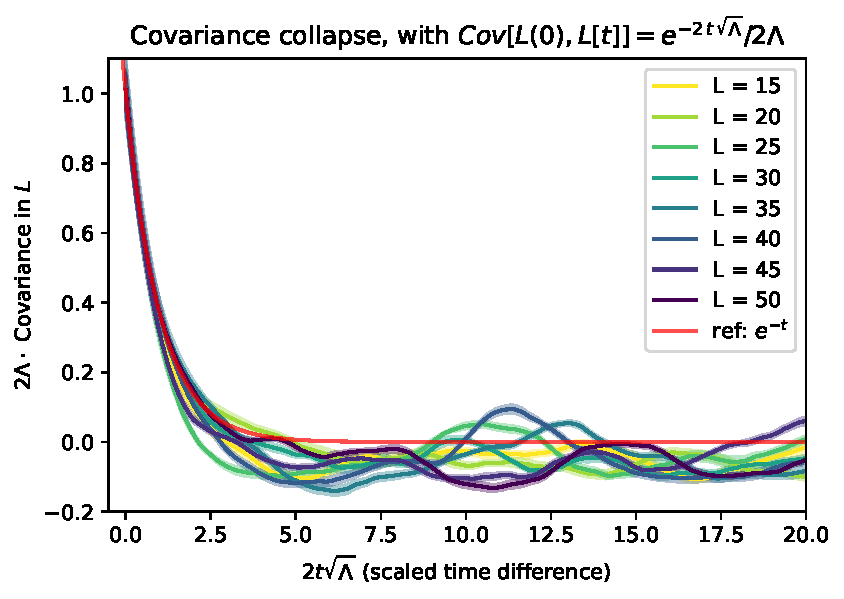
\includegraphics[width=\linewidth]{img/cov_collapsed.pdf}
        \caption{Scaled covariance with reference collapse function in red.}
        \label{fig:cov_collapsed}
    \end{minipage}
    \hfill
    \begin{minipage}[t]{0.49\linewidth}
        \centering
        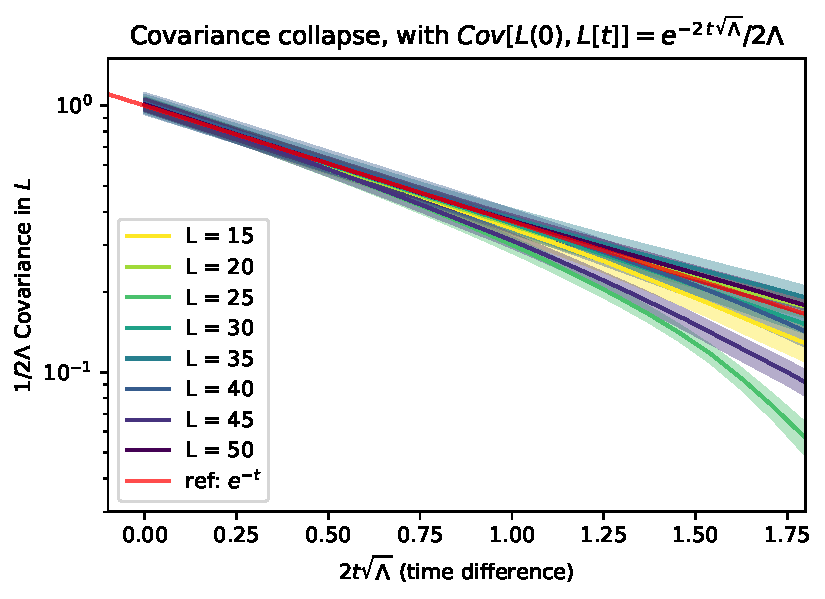
\includegraphics[width=\linewidth]{img/cov_collapsed_log.pdf}
        \caption{Logarithmic plot of scaled covariance.}
        \label{fig:cov_log_collapsed}
    \end{minipage}
\end{figure}
From these plots it is evident that the curves collapse well for small $t$, and that there are discrepancies for larger $t$ as expected.

To make this more quantitative we would want to fit the expected covariance with a general exponential function and compare the different estimation of $\Lambda$ as a result of this fit to each other and to $L$.
However, to be able to fit an exponential we need a large enough part of the covariance $\rho_\ell(t)$ for which $t$ can be considered `small'.
This means that $T$ needs to be larger for a given $L$ than we currently use.
It may also be possible to include higher order terms in the theoretical prediction of the covariance such that the theoretical prediction is valid for larger $t$.
Finally, since what we really want is to find the exponent of Eq. \eqref{eq:cov_ell} for small $t$ and this is equal to the slope at $t = 0$, we might be able to get a reasonable approximation of this slope by considering only the first few points and for example using spline interpolation or a polynomial fit to find the slope at $t=0$.

% \paragraph{Timothy's formula's}
Uit hoofdstuk 4.1 van arXiv:1203.3591 kun je afleiden dat in de continue
limiet met een tijdsinterval T en kosmologische constante $\Lambda$ de
covariantie van de ruimtelijke lengtes $L(t)$ in de limiet $T$ naar oneindig gegeven wordt door
\begin{equation}
    \text{Cov}\big(\ell(0), \ell(t)\big) = \Exp{\qty(\ell(0) - L)\qty(\ell(t) - L)}
    = \frac{1}{2\Lambda} e^{- 2\abs{t}\sqrt{\Lambda}}
\end{equation}
terwijl de verwachtingswaarde gelijk is aan
\begin{equation}
    \Exp{\ell(t)} = \frac{1}{\sqrt{\Lambda}} = L
\end{equation}
In deze limiet van grote $T$ is het de verwachting dat het niet veel
uitmaakt of het totale volume vastgezet wordt of dat er een
kosmologische constante genomen wordt (wat is de juiste relatie tussen
volume en $\Lambda$ in dit geval?).

Kun je deze covariantie zien in de data (tenminste voor $\abs{t} \ll T$)? En is
de constante in de $e$-macht daar ook gerelateerd aan $\Exp{L(t)}$?


\subsection{Discussion}\label{sec:discussion}
% Discussion of the interpretation and validity of the results
% Explaination of the difficulties in determining useful results
% Suggestions on improving these measurements
The measurements of the standard deviation $\sigma_\ell$ and of the covariance $\rho_\ell(t)$ agree with the theoretical predictions.
The main concern is the found results have a systematic underestimation of the standard deviation and thus also the covariance as explained due to finite $T$.
So, what should really be done to better understand the dependence of the results on $T$ is to repeat these measurements on different $T/L$ ratio's.
However, since the computation time increases with $N^{3/2}$, this put constraints on system sizes that can be simulated within a reasonable amount of time.

The determination of the equilibration time and correlation time is important to performing the simulation.
However, for this project great effort was taken to determine these times to reasonable accuracy to be able to predict $t_\text{eq}$ and $t_\text{cor}$ for any given $T$ and $L$.
Knowing the computational effort that went into determining these still rather inaccurate predictions, doing it this way is likely not worth it; it is much more fruitful to pick the system sizes one wishes to simulate carefully and determine the equilibration and correlation time for these systems specifically.
Unfortunately, we only later in the project realised what the interesting system sizes were, so we could not optimally use the determined $t_\text{eq}$ and $t_\text{cor}$ anyway.
Also, although we expect $t_\text{eq}$ to be independent of $T$, it should be checked to really make sure any system one does measurements one is thermalised.
If this is not the case and the total amount of measurements is low, the first few measurements could contribute to a significant error to the end results.

Finally, there are many more interesting observable to measure in 2D CDT, some of which are already discussed in section \ref{sec:observables}.
If the time permits it is highly recommended measuring some of these observables, but we could not find the time in this project to look at these.

%TODO%
% Maybe include the discussion of missing dependence on T for equilibration time?

\paragraph{from pre analysis} Later in the project we realised that the system sizes of interest were those where $L \ll T$, which is not the case for the systems the equilibration time and correlation time are measured for.
Re-computation of these quantities takes a lot of computational effort, and there was unfortunately not enough time available to do this.
Experience showed that taking $200 \, \text{sweeps}$ as burn-in time is also sufficient in this regime, and that the correlation time still scales with $N^{3/2}$ for a constant $T/L$ ratio.
The crude approximation for the correlation time does however not seem to be accurate for larger $T/L$ ratio's, as the correlation times seem lower than this estimate would suggest.

\section{Conclusion}
% Conclusions
Finally, there are many more interesting observable to measure in 2D CDT, some of which are already discussed in section \ref{sec:observables}.
If the time permits it is highly recommended measuring some of these observables, but we could not find the time in this project to look at these.

\printbibliography

\appendix
\section{Individual Contributions}
% explain briefly how you divided the work among each other on the various aspects: coding, data collection, data analysis, report writing
For the project we divided the work as follows:
\begin{itemize}
    \item \textit{Literature research}: Is done roughly equally
    \item \textit{Model design and programming}: Tom started with a vertex-based model, Jesse started a triangle-based model and we optimized that together. Tom designed the CLI, and Jesse the visualisation.
    \item \textit{Data analysis}: Jesse performed most of the data analysis, and collected all the data for the preliminary analysis. Tom collected the data for the main measurements and verified the validity of the data analysis.
    \item \textit{Report writing}: Writing is divided roughly equally, generally Tom was responsible for the Introduction and Methods, and Jesse for the Results with Discussion.
\end{itemize}
For a very detailed overview of the individual contribution, they can be found in the commits of the GitHub repository, see appendix \ref{sec:coderepo}

\section{Code and Data distribution} \label{sec:coderepo}
For this project we used a public GitHub repository (see \url{https://github.com/SirBlueRabbit/monte-carlo-CDT}) to share all project files and all relevant data.
For an overview of the contents of the repository see the \textsc{README}.


\end{document}